\subsection{Systemarchitektur}\label{subsec:systemarchitektur}
\subsubsection*{Abgrenzung}

Dieses Kapitel gibt einen Übersicht über die Systemarchitektur als ganzes. Die Architektur beschränkt sich dabei auf die
Anforderungen die innerhalb des Projektrahmens umgesetzt wurden. Komponenten für Teile die Out Of Scope gefallen sind,
werden hier nicht behandelt.

\subsubsection*{Übersicht}

Das cloudbasierte Praxisrufsystem wird in vier Komponenten unterteilt.
Im Zentrum steht eine cloudbasierte Applikation (Cloud Service) welche es ermöglicht Konfigurationen persistent zu verwalten und das Versenden von Benachrichtigungen anhand dieser Konfigurationen koordiniert.
Der Cloud Service benutzt einen externen Messaging Service zum Versenden von Benachrichtigungen. Dabei ist der Messaging Service lediglich für die Zustellung von Benachrichtigungen verantwortlich.
Zur Verwaltung der Konfigurationen wird ein Web Frontend (Admin UI) erstellt. Dieses bietet einem Administrator die Möglichkeit Konfigurationen aus dem Cloud Service zu lesen, erstellen, bearbeiten und löschen.
Die Konfigurationen die über Admin UI und Cloud Service erstellt wurden, werden schliesslich von einem Mobile Client. Mit dem Mobile Client kann der Benutzer Benachrichtigungen an andere Mobile Clients senden.
Welche Benachrichtigungen ein Mobile Client senden kann und an wen diese Benachrichtigungen zugestellt werden, wird anhand der Konfiguration aus dem Cloud Service bestimmt.

\begin{figure}[h]
    \centering
    \begin{minipage}[b]{1.0\textwidth}
        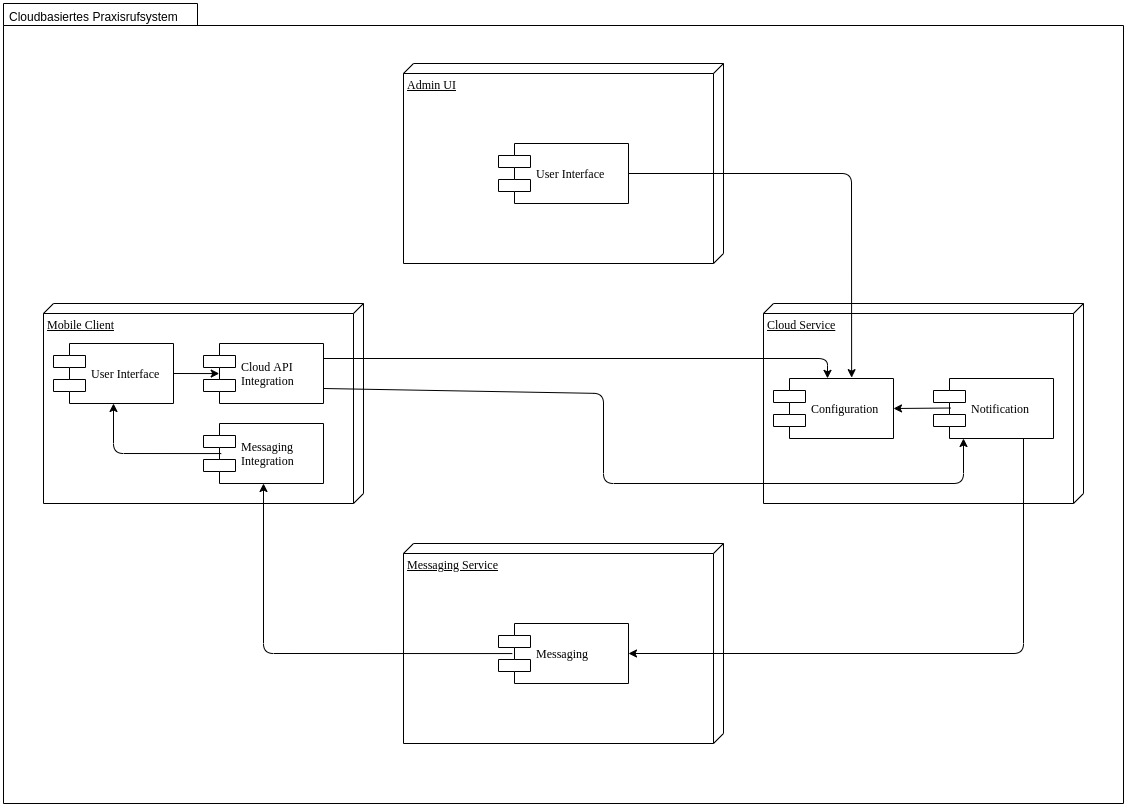
\includegraphics[width=\textwidth]{graphics/Component_System}
        \caption{System}
    \end{minipage}
\end{figure}

\clearpage
